     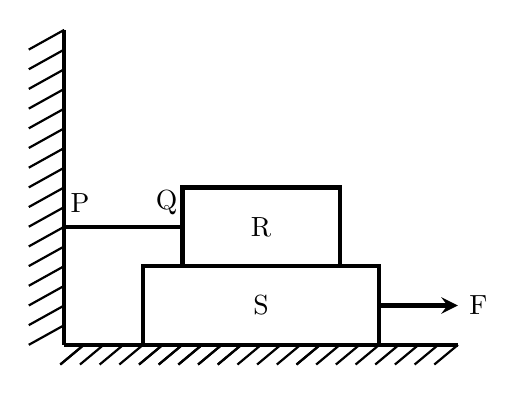
\begin{tikzpicture}
  
    \draw[ultra thick] (-1,4) -- (-1,0);
    \draw[ultra thick] (-1,0) -- (4,0);
\foreach \y in {0.25,0.5,0.75,1,1.25,1.5,1.75,2} {
        \draw[thick] (-1.45,\y-0.25) -- (-1,\y);
    }
   \foreach \y in {0.25,0.5,0.75,1,1.25,1.5,1.75,2} {
        \draw[thick] (-1.45,\y+2-0.25) -- (-1,\y+2);
    }
    \foreach \x in {-1,0,0.25,0.5,0.75,1,1.25,1.5,1.75,2} {
        \draw[thick] (\x-0.05,-0.25) -- (\x+0.25,0);
    }
    \foreach \x in {0,0.25,0.5,0.75,1,1.25,1.5,1.75,2} {
        \draw[thick] (\x-0.05-1,-0.25) -- (\x+0.25-1,0);
    }
     \foreach \x in {0,0.25,0.5,0.75,1,1.25,1.5,1.75} {
        \draw[thick] (\x-0.05+2,-0.25) -- (\x+0.25+2,0);
    }
    \draw[ultra thick] (0,0) rectangle (3,1) node[midway] {S};
    \draw[ultra thick] (0.5,1) rectangle (2.5,2) node[midway] {R};


    \draw[ultra thick] (-1,1.5) -- (0.5,1.5); 
    \draw[ultra thick] (0.5,1.5) -- (0.5,2);\node at (-0.8,1.8) {P};\node at(0.3,1.8) {Q};
    \draw[->, ultra thick,>=stealth] (3,0.5) -- ++(1,0) node[right] {F};
\end{tikzpicture}
